\documentclass{article}
\usepackage{graphicx,amssymb,amsmath,amsbsy,MnSymbol}

\usepackage[T1]{fontenc}        % pour les charactères accentués
\usepackage[utf8]{inputenc}

\setlength{\parindent}{0.0in}
\setlength{\parskip}{0.3in}
\setlength{\topmargin}{-0.4in}
\setlength{\topskip}{1in}    % between header and text
\setlength{\textheight}{8in} % height of main text
\setlength{\textwidth}{6in}    % width of text
\setlength{\oddsidemargin}{0.5in} % odd page left margin
\setlength{\evensidemargin}{0.5in} % even page left margin

\bibliographystyle{plain}

\pagenumbering{arabic}
\date{\today}
\title{Smooth object retrieval using Bag of Boundaries}
\author{Vadim Kantorov \& Nelle Varoquaux}
\begin{document}
\maketitle
\begin{abstract}

\end{abstract}

\section{Introduction}
Object recognition is one of the many very active field of vision. Extracting
viewpoints and lightning invariant descriptors is now done efficiently,
allowing performant commercial applications. \\
However, current methods fail on two type of objects: smooth objects and wiry
objects. We will focus on the smooth objects, using methods
\cite{Arandjelovic11} introduces: boundary descriptors. These new descriptors
focus on describing the form of the objects, allowing to retrieve objects
of same shape, but of different sizes and materials. \\
We will use the sculptures 6K dataset: it contains $6000$ pictures of
sculptures, mostly the work of Moore and Rodin, with groundtruth for twenty
of this sculptures. Most sculptures appear several times in the dataset, taken
from different points of views. As Henry Moore often made sculptures of the
same form in different materials, such as bronze and marble, this dataset is
pertinent to test shape and boundaries descriptors.

\section{Segmentation}
\section{Boundary descriptors}

\begin{figure}

\label{boundary-descriptors}
\begin{center}
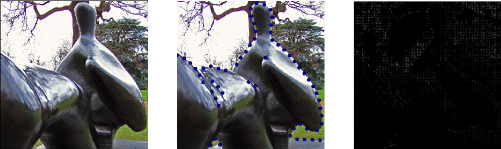
\includegraphics[width=350px]{images/desc.png}
\end{center}
\caption{Boundary descriptors are extracted on a sampled edge, at different
scale. A descriptor is composed of a HoG and a occupancy grid}
\end{figure}

% \caption{The foreground occupancy mask is a grid, where the value of each
% cell represents the ration of foreground pixels.}

\cite{Arandjelovic11} presents a new shape descriptors, invariant to texture
and color, but also lighting, scale and small viewpoints changes. It needs to
be local, in order to be robust to partial occlusions. \\
The boundary descriptors are formed of two descriptors: a Histogram of
Gradients (HoG) and a foreground mask occupancy grid.
\section{Results}
\section{Conclusion}

\bibliography{biblio.bib}

\end{document}
